\documentclass{article}
\usepackage[T1]{fontenc}
\usepackage{lmodern}
\usepackage{graphicx}
\usepackage{amsmath,amssymb}
\usepackage[a4paper,margin=2cm]{geometry}
\usepackage[absolute,overlay]{textpos}
\setlength{\TPHorizModule}{1mm}
\setlength{\TPVertModule}{1mm}
\usepackage[indonesian]{babel}
\usepackage{hyperref}
\setlength{\emergencystretch}{2em}
% unit: Halaman 11

\begin{document}

% === Halaman 11 (llm) ===

\section*{Penjelasan Analitik P + Q = R}

Persamaan garis g: \[ y = mx + c \]

\vspace{160.38mm}

Gradien garis g: \[ m = \frac{y_p - y_q}{x_p - x_q} \]

Perpotongan garis g dengan kurva $y^2 = x^3 + ax + b$ adalah:
\[ (mx + c)^2 = x^3 + ax + b \]

\vspace{50mm}

Koordinat Titik R:
\[
\begin{aligned}
x_r &= m^2 - x_p - x_q \\
y_r &= m(x_p - x_r) - y_p
\end{aligned}
\]

\vspace{10mm}
\hfill \textcolor{red}{Sumber gambar: Andreas Steffen, Elliptic Curve Cryptography}

% deskripsi: Grafik kurva eliptik dengan garis g yang memotong titik P, Q, dan -R, serta proyeksi titik -R ke titik R
% bbox normalisasi: [0.5150, 0.2300, 0.8650, 0.7700]
\begin{textblock*}{73.50mm}(108.15mm,68.31mm)
\noindent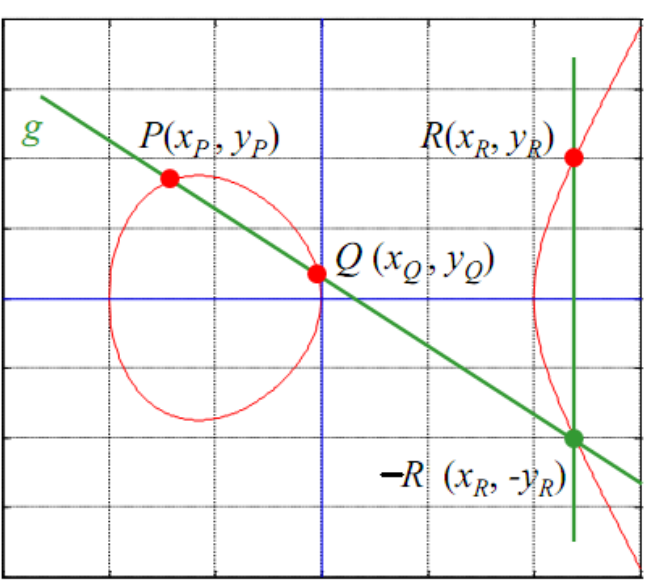
\includegraphics[width=73.50mm,height=160.38mm]{../../images/llm/page_011_img_01.png}%
\end{textblock*}

\end{document}
